Pasemos a confirmar lo que vimos teóricamente en la sección anterior.

Como vimos en la introducción, graficaremos los tiempos con el tamaño dela entrada en el eje $x$ y el cociente entre el tiempo de ejecución y el tamaño de la entrada en el eje $y$, si esto da una constante, significará que la cota que encontramos es ajustada, si tiende a 0, que es holgada, por definición de $\Theta(f(n))$ y $O(f(n))$ respectivamente.

Para testear el algoritmo utilizamos el algoritmo de generación de grafos al azar descripto en el ap\'endice. Tuvimos que generar grafos realmente pequeños (no mas de 10 nodos cada uno), dada la naturaleza exponencial del algoritmo exacto.

Pasemos a ver los resultados.

\begin{figure}[H]
 \centering
	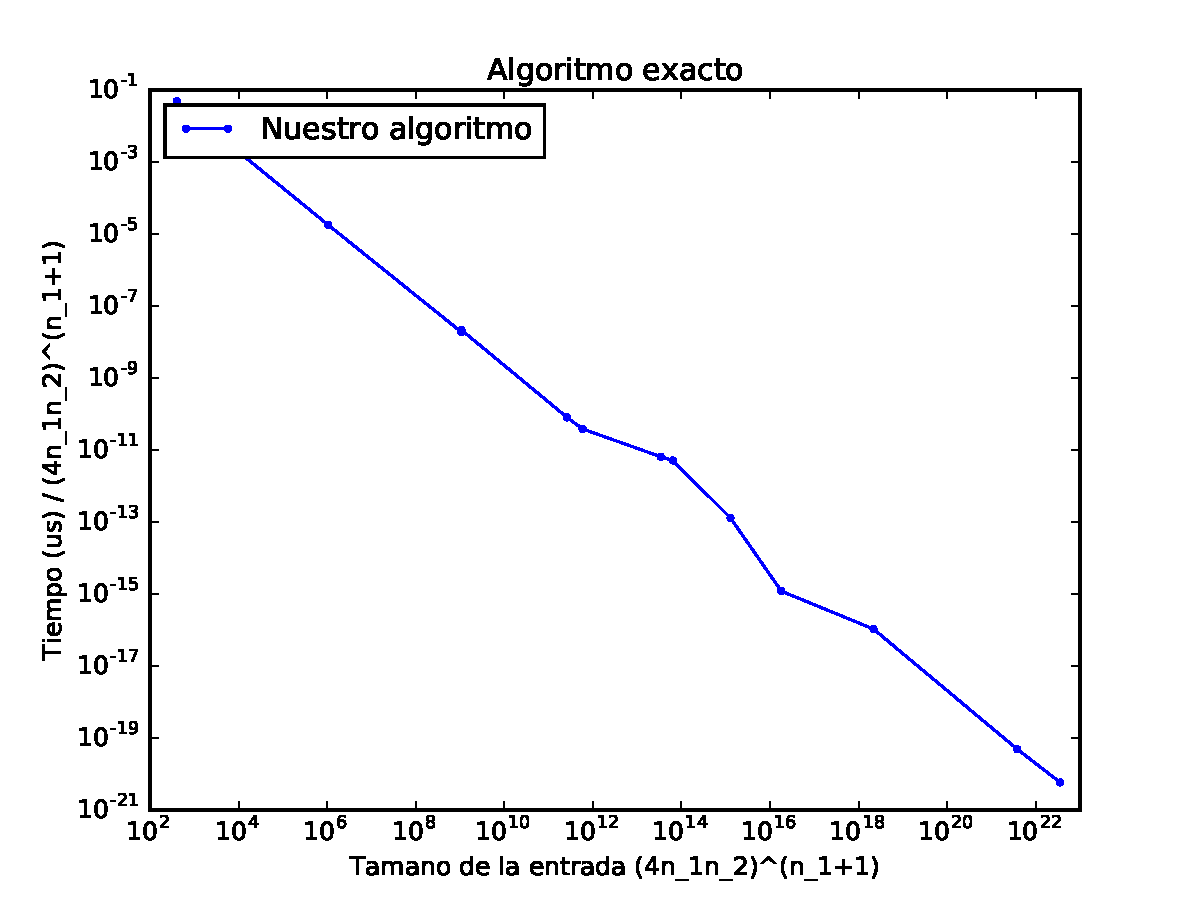
\includegraphics[width=0.9\textwidth]{graficos/problema_2/tiempos_1.pdf}
	\caption{}
	\label{fig:problema2-1}
\end{figure}

Como vemos, el ratio entre tiempo y tamaño de entrada tiende a 0, por lo que, además de ser correcta la complejidad que dimos, tambi\'en confirmamos que es holgada, como conjeturamos en la sección anterior, durante su derivación.

Otro experimento que siempre vale la pena hacer es el de fijar una de las variables de entrada y mover el resto, para ver que el algoritmo se comporte como esperamos. En este caso la única variable que vale la pena fijar es $n_1$, dado que si se fija $n_2$ el gráfico de la complejidad es exactamente igual al anterior.

El caso interesante es el caso en el que $n_1$ está fijo, dado que aquí la complejidad, según lo que vimos, debería ser polinomial. Recordemos que siempre pasa que $n_1 < n_2$, por lo que esto nos habla de como se van a comportar el algoritmo si fijamos el grafo mas pequeño.

Veamos los resultados.


\begin{figure}[H]
 \centering
	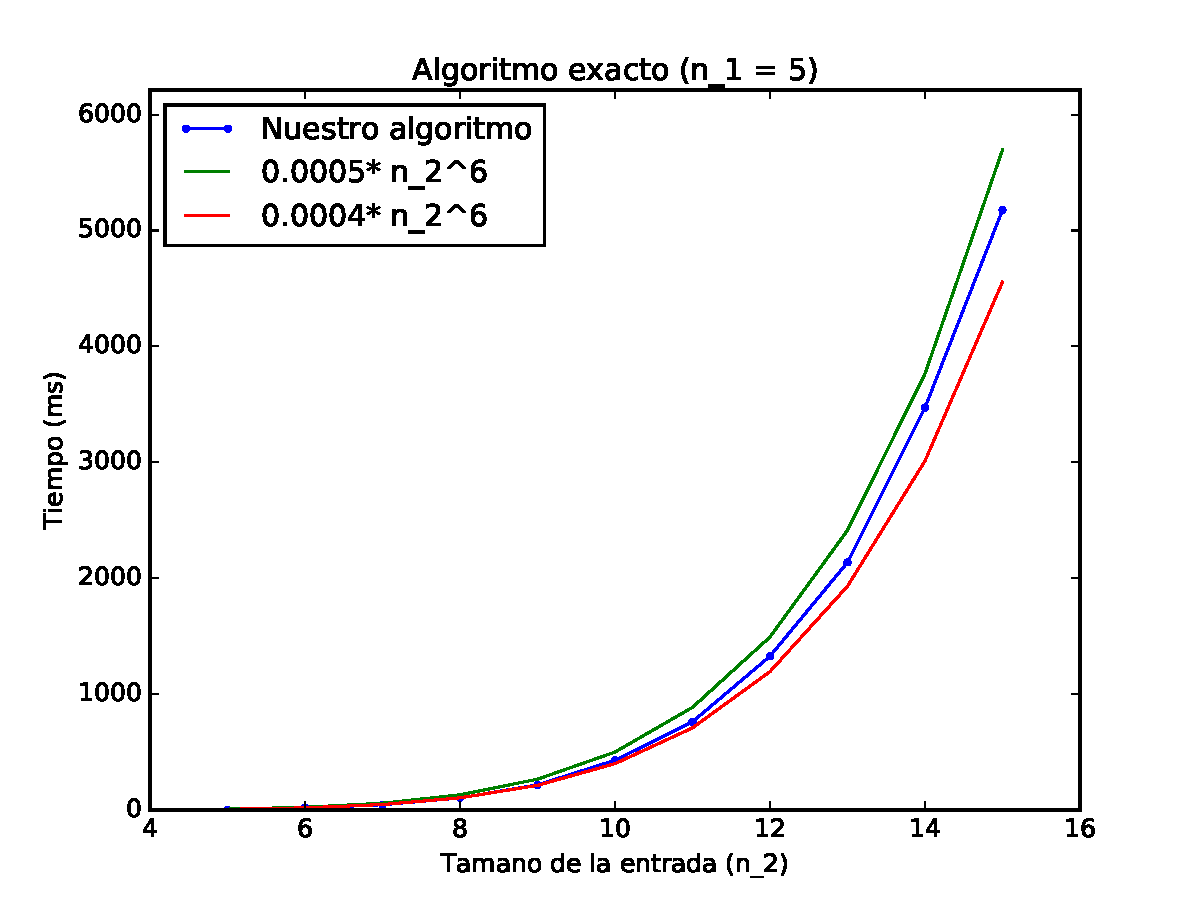
\includegraphics[width=0.9\textwidth]{graficos/problema_2/tiempos_2.pdf}
	\caption{}
	\label{fig:problema2-2}
\end{figure}

Como vemos, se confirman nuestras expectativas: el algoritmo es polinomial con el exponente esperado.
Es más, la cota es ajustada, de hecho es uno de los experimentos con resultado más limpio que obtuvimos en todo el trabajo.


